\documentclass[letterpaper,11pt]{article}
\usepackage{amsmath}
\usepackage{moreverb}
\usepackage{amssymb}
\usepackage{graphicx}
\usepackage{mathtools}
\usepackage{tikz}
\usepackage{pgfplots}
\usepackage{float}
\usetikzlibrary{arrows,shapes, positioning}
\DeclarePairedDelimiter\floor{\lfloor}{\rfloor}
\let\biconditional\leftrightarrow
\addtolength{\oddsidemargin}{-.875in}
\addtolength{\evensidemargin}{-.875in}
\addtolength{\textwidth}{1.75in}
\addtolength{\topmargin}{-.875in}
\addtolength{\textheight}{1.75in}
\newenvironment{customlegend}[1][]{%
    \begingroup
    % inits/clears the lists (which might be populated from previous
    % axes):
    \csname pgfplots@init@cleared@structures\endcsname
    \pgfplotsset{#1}%
}{%
    % draws the legend:
    \csname pgfplots@createlegend\endcsname
    \endgroup
}%

% makes \addlegendimage available (typically only available within an
% axis environment):
\def\addlegendimage{\csname pgfplots@addlegendimage\endcsname}

\pgfkeys{/pgfplots/number in legend/.style={%
        /pgfplots/legend image code/.code={%
            \node at (0.295,-0.0225){#1};
        },%
    },
}

\title{Distributed Systems -- Deliverable 1}
\author{Jacob Errington (260636023) \\ Alexandre Laporte (260635979)}
\date{6 October 2015}

\begin{document}

\maketitle

\section*{Web Services}

The design of the webservices component of the deliverable is centered on
creating a middleware manager. In order to achieve this we created
the \texttt{MiddlewareResourceManager} class implementing the same interface as
the backend servers. Hence, from a client's perspective, it is
indistinguishable from a backend server.

Internally, the middleware dispatches incoming requests to a backend server
according to the type of request. Once the backend server's reply is received,
it is transmitted back to the client.

More complex requests such as reservations require additional work from the
middleware server. For example, in order to reserve a flight, the middleware
must first ensure that the customer exists by querying the customer server,
and then reserves the flight by sending a request to the flight server. The
case of printing a bill is even more complicated as it requires querying every
backend server once.

\begin{figure}[H]
    \centering

    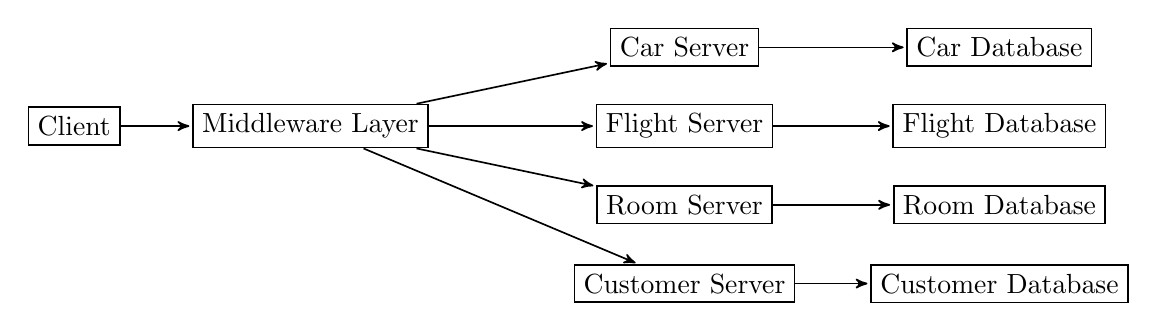
\begin{tikzpicture}[->,>=stealth',shorten >=1pt,auto,node distance=1cm,semithick]
        \node[draw] (rect) (A)                            {Client};
        \node[draw] (rect) (B) [right of=A,xshift=2cm]    {Middleware Layer};
        \node[draw] (rect) (C) [right of=B,xshift=3.75cm] {Flight Server};
        \node[draw] (rect) (D) [above of=C]               {Car Server};
        \node[draw] (rect) (E) [below of=C]               {Room Server};
        \node[draw] (rect) (F) [below of=E] 	          {Customer Server};
        \node[draw] (rect) (G) [right of=C, xshift=3cm]   {Flight Database};
        \node[draw] (rect) (H) [right of=D, xshift=3cm]   {Car Database};
        \node[draw] (rect) (I) [right of=E, xshift=3cm]   {Room Database};
        \node[draw] (rect) (J) [right of=F, xshift=3cm]   {Customer Database};

        \path
        (A) edge                node {} (B)
        (B) edge                node {} (C)
            edge                node {} (D)
            edge                node {} (E)
            edge		        node {} (F)
        (C) edge                node {} (G)
        (D) edge                node {} (H)
        (E) edge                node {} (I)
        (F) edge 		        node {} (J);
    \end{tikzpicture}

    \caption{
        The architecture of our system uses a middleware server to contact
        independent backend servers to perform tasks related to different
        types of reservable items. Each backend server uses a database to
        ensure the internal consistency of its data as well as to guarantee
        that concurrent writes can be performed reliably.
        However, since each backend server has its own database, data
        consistency across databases is managed by the middleware.
    }
\end{figure}

\section*{Database architechture}

As persistent backing stores for the data in this system, we choose to use
relational databases. This allows us to effectively represent certain
relationships between the different types of data in the system, in particular
the reservations of items by the customers.

Each backend server is equipped with a database to store a list of items as
well which items are reserved and by whom. However, because the customer
information is maintained by a separate resource manager, foreign key
contraints on the customer identifier cannot be made. Hence, unless certain
precautions are made by the middleware server, it may arise that items become
reserved by a customer that does not exist.

Nonetheless, the database schema is programmed to guarantee that certain
undesirable scenarios are impossible, even under heavy concurrent loads. For
example, thanks to the judicious use of foreign key and unique constraints,
items cannot be reserved more than once per customer nor can items be reserved
by more than one customer at once.

\section*{TCP Sockets}

The overall architecture of the TCP sockets application is identical to the
structure of the web services application; we merely replace the HTTP transport
with our own transport. This introduces many new challenges. In particular, we
concern ourselves with efficiently managing multiple concurrent connections as
well as transferring objects over the network.

At the core of both the middleware and backend servers, there is a tight loop
that accepts incoming connections. Upon each new connection being established,
a handler is created for that connection and is run in a different thread. We
use a pool with a fixed number of threads based on the number of logical
processors on the machine. Consequently, new connections may be accepted while
requests are being handled in these worker threads, and many requests may be
processed concurrently.

Objects are sent over the network using Java's built-in serialization
capabilities. However, we pass only two types of objects over the network.

\begin{description}
    \item[Request.] A request object represents a remote method invocation on
        the recipient server's ResourceManager. As such, it simply contains the
        name of the method to invoke, an array of objects to use as parameters,
        and some metadata on the parameters. The request object implements a
        method using reflection to invoke the method on a provided object
        implementing the resource manager interface. This allows us to remain
        agnostic about the precise implementation of this interface, and
        consequently, we can use identical request objects for both
        client-middleware and middleware-backend communications.

    \item[Response.] A response object represents the return value of the
        remote method invocation. Since remote method invocations may abruptly
        fail, we bracket the method calls with exception handlers that
        package the exception into the response object and return it to the
        client, where it is thrown again. This allows exceptions to
        transparently be thrown across the network, and prevents exceptions
        raised by event handler code from crashing the socket accept loop.
        However, clients and the middleware must take care to check for these
        exceptions.
\end{description}

\begin{figure}[H]
    \centering

    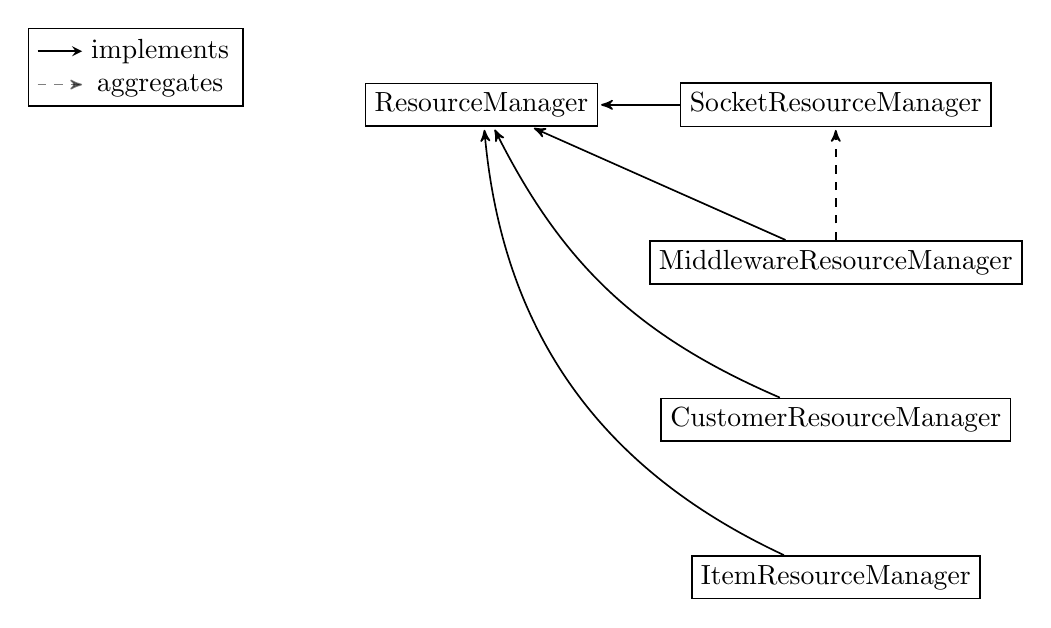
\begin{tikzpicture}[->,>=stealth',shorten >=1pt,auto,node distance=2cm,semithick]
        \node[draw] (rect) (B) [xshift=4cm] {ResourceManager};
        \node[draw] (rect) (A) [right of=B, xshift=2.5cm]                {SocketResourceManager};
        \node[draw] (rect) (E) [below of=A]      {MiddlewareResourceManager};
        \node[draw] (rect) (C) [below of=E]      {CustomerResourceManager};
        \node[draw] (rect) (D) [below of=C]      {ItemResourceManager};
        \path
        (A) edge node {} (B)
        (C) edge[bend left=20] node {} (B)
        (D) edge[bend left=30] node {} (B)
        (E) edge node {} (B)
        (E) edge[dashed]       node {} (A)
        ;

        \begin{customlegend}[
            legend entries={ % <= in the following there are the entries
                implements,
                aggregates
            }
        ] % <= to define position and font legend
          % the following are the "images" and numbers in the legend
            \addlegendimage{-stealth,black,opacity=1}
            \addlegendimage{black,dashed,opacity=0.5}
        \end{customlegend}
    \end{tikzpicture}

    \caption{
        Each component of the system is represented by a class implementing the
        \texttt{ResourceManager} interface, which defines the basic set of
        capabilities that can be performed on reservable items.
        Backend servers use a \texttt{CustomerResourceManager} or a
        \texttt{ItemResourceManager} to perform actions on their respective
        backing store, using a pool of database connections, according to the
        type of data that they manage.
        Clients use a \texttt{SocketResourceManager} to send \texttt{Request}
        objects representing the remote methods to call.
        The middleware server's \texttt{MiddlewareResourceManager} aggregates a
        number of \texttt{SocketResourceManager}s, one for each connected
        backend server.  Many requests received by the middleware simply need
        to be forwarded to the appropriate backend server, but some requests
        require aggregating data across all nodes in order to present summary
        information to the client.
    }
\end{figure}

\end{document}
